
    A typical memory representation of a C program consists of the following sections.
    \begin{enumerate}
        \item Text/Code segment  
        \item Initialized data segment 
        \item Uninitialized data segment  (bss)
        \item Heap 
        \item Stack
    \end{enumerate}

    \begin{figure}[H]
        \begin{center}
            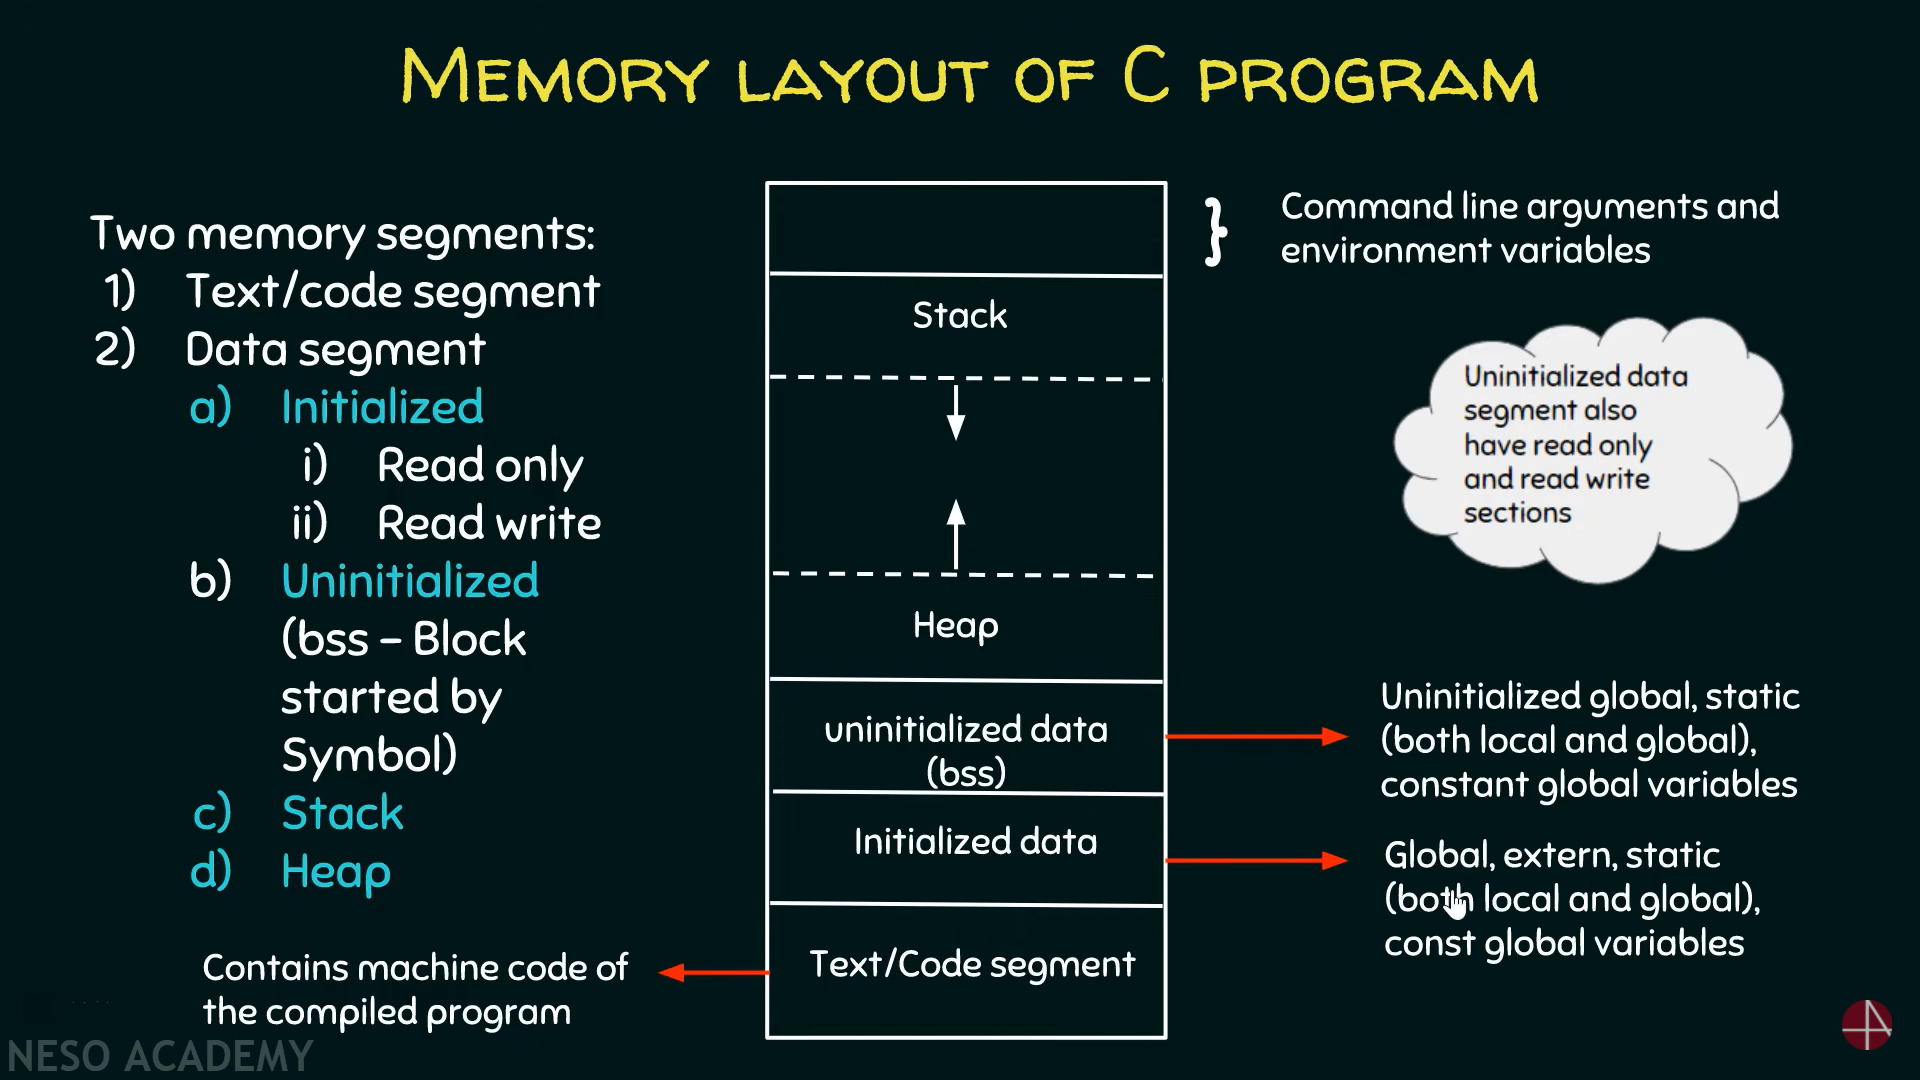
\includegraphics[width=0.6\textwidth]{images/memoryLayoutC.png}
            \caption{Memory Layout of C program}
            \label{memoryLayoutC}
        \end{center}
    \end{figure}

    C program gets stored into not one but multiple sections of the memory. A typical memory layout of a running process is as follows:
    \subsection{Text/Code segment}
    \begin{itemize}
        \item A text segment, also known as a code segment or simply as text, contains machine code of the compiled program or executable instructions.
        \item The text segment is often read-only, to prevent a program from accidentally modifying its instructions.        
        \item As a memory region, a text segment may be placed below the heap or stack in order to prevent heaps and stack overflows from overwriting it.         
        \item Usually, the text segment is sharable so that only a single copy needs to be in memory for frequently executed programs, such as text editors, the C compiler, the shells, and so on. 
    \end{itemize}   
    
    \subsection{Initialized Data Segment}
    \begin{itemize}
        \item Initialized data segment, usually called simply the Data Segment. 
        \item A data segment is a portion of the virtual address space of a program, which contains the global, extern, static (local and global), and const global variables that are initialized by the programmer.
        \item Note that, the data segment is not read-only, since the values of the variables can be altered at run time.    
        \item This segment can be further classified into the read-only (for const-s) area and the read-write sections.
    \end{itemize}
    
    \subsection{Uninitialized Data Segment}
    \begin{itemize}
        \item Uninitialized data segment often called the "bss" segment, named after an ancient assembler operator that stood for "block started by symbol".
        \item Uninitialized data segment contains all uninitialized global, static(local and global), and constant global variables.
        \item Data in this segment is initialized by the kernel to arithmetic 0 before the program starts executing.    
        \item This segment is also further classified into read-only (for const-s) area and read-write sections.             
    \end{itemize}
    
    \subsection{Stack}
    The stack area traditionally adjoined the heap area and grew in the opposite direction; when the stack pointer met the heap pointer, free memory was exhausted. (With modern large address spaces and virtual memory techniques they may be placed almost anywhere, but they still typically grow in opposite directions.)

    The stack area contains the program stack, a LIFO structure, typically located in the higher parts of memory. On the standard PC x86 computer architecture, it grows toward address zero; on some other architectures, it grows in the opposite direction. A "stack pointer" register tracks the top of the stack; it is adjusted each time a value is "pushed" onto the stack. The set of values pushed for one function call is termed a "stack frame"; A stack frame consists at minimum of a return address.

    Stack, where automatic variables are stored, along with information that is saved each time a function is called. Each time a function is called, the address of where to return to and certain information about the caller's environment, such as some of the machine registers, are saved on the stack. The newly called function then allocates room on the stack for its automatic and temporary variables. This is how recursive functions in C can work. Each time a recursive function calls itself, a new stack frame is used, so one set of variables doesn't interfere with the variables from another instance of the function.
    
    \subsection{Heap}
    Heap is the segment where dynamic memory allocation usually takes place.
    
    The heap area begins at the end of the BSS segment and grows to larger addresses from there. The Heap area is managed by malloc, realloc, and free, which may use the brk and sbrk system calls to adjust its size (note that the use of brk/sbrk and a single "heap area" is not required to fulfill the contract of malloc/realloc/free; they may also be implemented using mmap to reserve potentially non-contiguous regions of virtual memory into the process' virtual address space). The Heap area is shared by all shared libraries and dynamically loaded modules in a process.